\documentclass[12pt]{article}
\usepackage[a4paper, top=2.5cm, bottom=2.5cm, left=1.5cm, right=1.5cm]{geometry}
\usepackage{amsmath, amsfonts, amssymb, mathtools}
\usepackage{fancyhdr, setspace, parskip}
\usepackage{graphicx, caption, subfig, array, multirow}
\usepackage{hyperref, enumitem, cancel}
\usepackage[T1]{fontenc}
\usepackage{tgtermes}
\usepackage[dvipsnames]{xcolor}
\usepackage{tocloft}
\usepackage{titlesec}
\usepackage{lipsum}  

\definecolor{DarkBlue}{RGB}{10, 0, 80}

% Hyperlink setup
\hypersetup{
    colorlinks=true,
    linkcolor=DarkBlue,
    filecolor=BrickRed,      
    urlcolor=RoyalBlue,
}


% Header and footer customization
\fancyhead{}
\fancyhead[L]{
{\fontfamily{lmss}{\color{DarkBlue}
\textbf{\leftmark}
}}
}
\fancyhead[R]{
{\fontfamily{ppl}\selectfont {\color{DarkBlue}
{Deep RL [Spring 2025]}
}}
}

\fancyfoot{}
\fancyfoot[C]{
{\fontfamily{lmss}{\color{BrickRed}
\textbf{\thepage}
}}
}

\renewcommand{\sectionmark}[1]{ \markboth{\thesection\quad #1}{} }

\renewcommand{\headrule}{{\color{BrickRed}\hrule width\headwidth height 0.5pt}}
\renewcommand{\footrulewidth}{0pt}


% Table of Contents customizations
\renewcommand{\cftsecafterpnum}{\vskip6pt}
\renewcommand{\cftsubsecafterpnum}{\vskip3pt}
\renewcommand{\cftsubsubsecafterpnum}{\vskip3pt}
\renewcommand{\cftsecfont}{\sffamily\large}
\renewcommand{\cftsubsecfont}{\sffamily}
\renewcommand{\cftsubsubsecfont}{\sffamily}
% \renewcommand{\cftsecdotsep}{1}
\renewcommand{\cftsubsecdotsep}{1}
\renewcommand{\cftsubsubsecdotsep}{1}


% Section title styles
\titleformat*{\section}{\LARGE\bfseries\color{DarkBlue}}
\titleformat*{\subsection}{\Large\bfseries\color{DarkBlue}}
\titleformat*{\subsubsection}{\large\bfseries\color{DarkBlue}}

\definecolor{light-gray}{gray}{0.95}
\newcommand{\code}[1]{\colorbox{light-gray}{\texttt{#1}}}

% Start of the document
\pagestyle{fancy}

%%%%%%%%%%%%%%%%%%%%%%%%%%%%%%%%%%%%%%%%%%%%%%%%%

\begin{document}

\pagenumbering{gobble}
\thispagestyle{plain}

\begin{center}

\vspace*{-1.5cm}
\begin{figure}[!h]
    \centering
    
\includegraphics[width=0.7\linewidth]{figs/cover-std.png}
\end{figure}

{
\fontfamily{ppl}

{\color{DarkBlue} {\fontsize{30}{50} \textbf{
Deep Reinforcement Learning
}}}

{\color{DarkBlue} {\Large
Professor Mohammad Hossein Rohban
}}
}


\vspace{20pt}

{
\fontfamily{lmss}


{\color{RedOrange}
{\Large
Homework 4:
}\\
}
{\color{BrickRed}
\rule{12cm}{0.5pt}

{\Huge
Advanced Methods in RL
}
\rule{12cm}{0.5pt}
}

\vspace{10pt}

{\color{RoyalPurple} { \small By:} } \\
\vspace{10pt}

{\color{Blue} { \LARGE Ali Ghasemzadeh } } \\
\vspace{5pt}
{\color{RoyalBlue} { \Large 401106339 } }


\vspace*{\fill}
\begin{center}
\begin{tabular}{ccc}
    
\includegraphics[width=0.14\linewidth]{figs/sharif-logo.png} & 
\includegraphics[width=0.14\linewidth]{figs/riml-logo.png} & 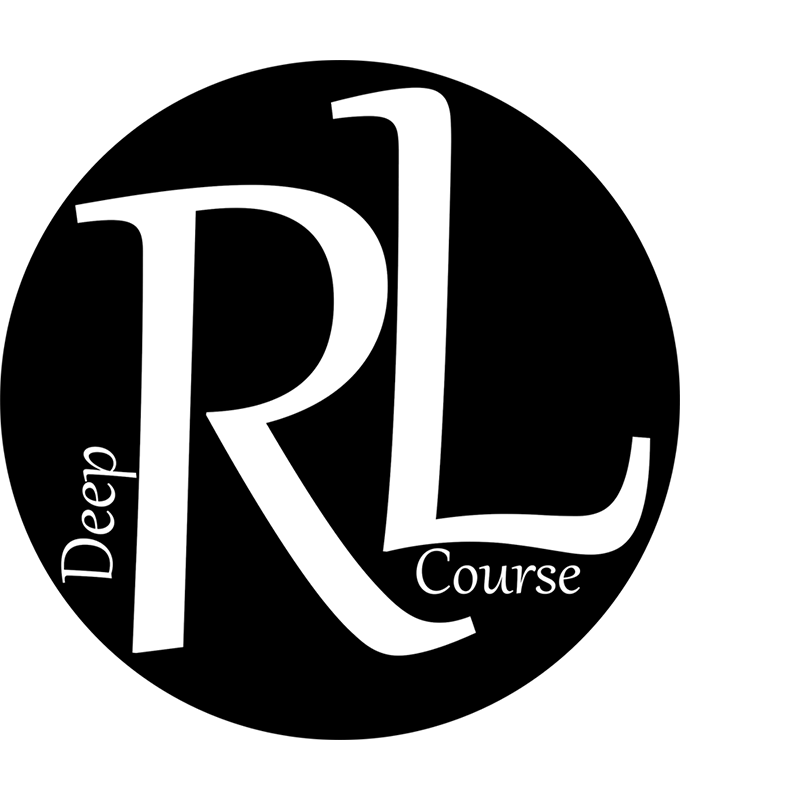
\includegraphics[width=0.14\linewidth]{figs/dlr-logo.png} \\
\end{tabular}
\end{center}


\vspace*{-.25cm}

{\color{YellowOrange} {
\rule{10cm}{0.5pt} \\
\vspace{2pt}
\large Spring 2025}
}}
\vspace*{-1cm}

\end{center}

%%%%%%%%%%%%%%%%%%%%%%%%%%%%%%%%%%%%%%%%%%%%%%%%%


\newpage
\pagenumbering{gobble}
\thispagestyle{plain}
{\fontfamily{lmss}\selectfont {\color{BrickRed} \textbf{\tableofcontents} }}

{\fontfamily{lmss}\selectfont {\color{DarkBlue}

\subsection*{Grading}

The grading will be based on the following criteria, with a total of 100 points:

\[
\begin{array}{|l|l|}
\hline
\textbf{Task} & \textbf{Points} \\
\hline
\text{Task 1: PPO} & 25 \\
\text{Task 2: DDPG} & 20 \\
\text{Task 3: SAC} & 25 \\
\text{Task 4: Comparison between SAC \& DDPG \& PPO} & 20 \\
\hline
\text{Clarity and Quality of Code} & 5 \\
\text{Clarity and Quality of Report} & 5 \\
\hline
\text{Bonus 1: Writing your report in Latex } & 10 \\
\hline
\end{array}
\]

}



%%%%%%%%%%%%%%%%%%%%%%%%%%%%%%%%%%%%%%%%%%%%%%%%%

\newpage
\pagenumbering{arabic}

{\fontfamily{lmss}\selectfont {\color{DarkBlue}

\section{Task 1: Proximal Policy Optimization (PPO) [25]}


\subsection{Question 1:} What is the role of the actor and critic networks in PPO, and how do they contribute to policy optimization? \\
\textbf{Actor network} represent the policy $\pi_{\theta}(a|s)$ which maps the state s to the action a, it decides what action to take in a given state.\\ in the PPO the actor is updated to improve the probability of actions that lead to higher advantages. and PPO uses a cliped surrogate objective to update the actor in a constrained manner, preventing large unstabe policy updates.\\ 
$L^{CLIP}(\theta) = \mathbb{E}_t[min (r_t(\theta)A_t, clip(r_t(\theta), 1-\epsilon, 1+\epsilon)A_t)]$ where $r_t(\theta) = \frac{\pi_{\theta}(a_t|s_t)}{\pi_{\theta_{old}}(a_t|s_t)}$ and $A_t$ is the advantage estimate.\\
\textbf{Critic netwok} approximate the value function $V^{\pi}(s)$ estimated expected future rewards from the state s, it evaluate actions by providing a baseline to compute the advantage function $A_t = R_t - V^{\pi}(s_t)$ and the critic provides feedback about how good an action was compared to the expected outcome. it is trained to minimize $L^{value} = (V_{\pi}(s_t) - R_t)^2$
\subsection{Question 2:} PPO is known for maintaining a balance between exploration and exploitation during training. How does the stochastic nature of the actor network and the entropy term in the objective function contribute to this balance?\\
The actor Network in PPO defines a stochastic policy $\pi_{\theta}(a|s)$ meaning it outputs a probability distribution over possible actions, not just a single action. in the discrete outputs a softmax over action logits, and in the continuous action space outputs mean and variance of a guassian distribution, so since the actions are sampled from this distribution, the agent tries different actions-even ones with lower probabilities and this randomness helps the agent explore new possibilities especially early training. then as the agent learns, the distribution gets sharper(less variance) increasingly favoring high reward actions thus the agent gradually exploits what it has learned, but retains some exploratory behavior due to having distribution.\\
PPO often adds an entropy bonus to the total loss function : 
$L^{total} = L^{CLIP} + \beta H - L_{critic} $ where H is the entropy bonus and $\beta$ is a small coefficent.\\
entropy measures the randomness in the action distribution and high entropy means more randomness and more exploration, by rewarding high entropy the entropy bonus encourages exploration and prevents the policy from collapsing too early into deterministic behavior. in the training process it make the agent to learn better actions so entropy naturally decreases and the entropy bonus can be annealed (you can gradually reduced it) to allow more exploitation later.\\
\subsection{Question 3:} When analyzing the training results, what key indicators should be monitored to evaluate the performance of the PPO agent?\\
it is crucial to monitor learning process and stability:\\
\textbf{episode return} is the most direct measure of how well the agent is performing the task,
for example upward trend indicates learning and improvement, Plateau may suggest convergence or need for tuning, high variance could mean unstable learning or too much exploration.
\textbf{policy loss} reflects how much the policy is changing, for example small values indicates steady updates, very large spikes or near-zero for long periods could signal unstable training or policy stagnation.
\textbf{value loss} a good value estimate helps the actor make better decisions. for example decreasing over time show critic is learning and high or unstable values indicates poor value estimation-can affect policy learning.
\textbf{entropy} indicates the exploration level and for exampe high early decreasing gradually means healthy exploration-exploitation balance, too low too early might mean that the agent permaturely exploiting, risking getting stuck, too high for to long could mean over-exploration and slow convergence.
we also have a lot of other parameters too.


\newpage

\section{Task 2: Deep Deterministic Policy Gradient (DDPG) [20]}

\subsection{Question 1:}

What are the different types of noise used in DDPG for exploration, and how do they differ in terms of their behavior and impact on the learning process?\\ 
we can use different noises like Ornstein-Uhlenbeck which generates emporally correlated noise with a tendency to revert to a mean and cause the sequence of actions to be smoother, it is usefule in the environments where cosecutive actions should be correlated, aiding the discovery of rewarding action sequences, we can also use guassian noise and it Provides uncorrelated, random perturbations by sampling independently from a normal distribution at each timestep, it is Simpler to implement and has been found effective in many scenarios, though it may lead to less smooth exploration compared to OU noise. we can also use Parameter Space Noise that Perturbs the parameters of the policy network itself, leading to consistent changes in the agent's behavior over entire episodes, it  Encourages more structured exploration and has been shown to improve performance in certain environments.\\
in this homework it uses gaussian noise in the DeterministicPolicy class.

\vspace*{0.3cm}

\subsection{Question 2:}

What is the difference between PPO and DDPG regarding the use of past experiences?\\
PPO is an on-policy algorithm, meaning it learns from data generated by the current version of the policy. After the policy is updated, previous experiences become outdated and are no longer used for learning. This approach ensures that the learning process is stable and consistent with the current policy's behavior. \\
In contrast, DDPG is an off-policy algorithm that utilizes a replay buffer to store past experiences. This allows DDPG to learn from data collected at different times, improving sample efficiency and enabling the reuse of experiences across multiple training iterations.

\newpage

\section{Task 3: Soft Actor-Critic (SAC) [25]}

\subsection{Question 1:}
\textbf{why do we use two Q-networks to estimate Q-values?}
\newline
SAC employs two separate Q-networks to estimate action values. This "double Q-learning" approach mitigates the risk of overestimating Q-values—a common issue when using a single network—by taking the minimum value predicted by the two networks. This conservative estimate leads to more stable and reliable learning. 


\vspace*{0.3cm}

\subsection{Question 2:}
\textbf{what is the temperature parameter($\alpha$), and what is the benefit of using a dynamic $\alpha$ in SAC?}
\newline
The temperature parameter, $\alpha$, balances the trade-off between maximizing expected returns and promoting policy entropy (randomness in action selection). A higher $\alpha$ encourages more exploration by favoring entropy, while a lower $\alpha$ emphasizes exploitation of known rewarding actions.\\
Allowing $\alpha$ to adjust dynamically during training enables the agent to automatically find an optimal balance between exploration and exploitation. This adaptability can lead to improved performance across various tasks without the need for manual tuning.


\vspace*{0.3cm}

\subsection{Question 3:}
\textbf{what is the difference between evaluation mode and training mode in SAC?}
\newline
In training mode, SAC's policy is stochastic, introducing randomness to encourage exploration. During evaluation mode, the policy typically becomes deterministic, selecting actions with higher certainty to assess learned performance accurately. This distinction ensures that the evaluation reflects the policy's true capabilities without the variability introduced during exploration. 


\newpage

\section{Task 4: Comparison between SAC \& DDPG \& PPO [20]}

\subsection{Question 1:}
\textbf{Which algorithm performs better in the \texttt{HalfCheetah} environment? Why?}
\newline
Compare the performance of the PPO, DDPG, and SAC agents in terms of training stability, convergence speed, and overall accumulated reward. Based on your observations, which algorithm achieves better results in this environment?\\
SAC is more stable and converges faster than others and it also gets more reward than PPO and a little more reward than DDPG. also we can see PPO gets about 3000 in this env but DDPG and SAC get about 10000 and we can also see that we are more stable with SAC in training, also SAC converges faster than others, DDPG converges fast but it risks instablity, overall : \\
PPO acheives competitive rewards but doesn't reach the highest reward.\\
DDPG is capable of high rewards and reach a very high reward but with considerable cariability due to training instability.\\
SAC consistently reach a high reward with lower variance across training runs.

\subsection{Question 2:}
\textbf{How do the exploration strategies differ between PPO, DDPG, and SAC?}
\newline
Compare the exploration mechanisms used by each algorithm, such as deterministic vs. stochastic policies, entropy regularization, and noise injection. How do these strategies impact learning in environments with continuous action spaces?\\
PPO utilizes a stochastic approach, where actions are sampled from a probability distribution. This inherent randomness encourages exploration, allowing the agent to discover and learn from different actions and to further promote exploration, PPO incorporates an entropy bonus in its objective function. This mechanism discourages premature convergence to deterministic policies, maintaining a degree of randomness that aids in thorough environment exploration.\\
DDPG employs a deterministic policy, selecting specific actions without inherent randomness. To facilitate exploration, it adds noise—commonly from an guassian process—to these actions during training. This approach enables the agent to explore the action space while learning precise control strategies.\\
SAC combines a stochastic policy framework with an entropy term in its reward function. This combination encourages the agent to balance the pursuit of high rewards with the maintenance of action diversity, effectively managing the exploration-exploitation trade-off.\\

In PPO its stochastic nature and entropy regularization promote broad exploration and can be beneficial in complex environments.\\
In DDPG policy augmented with noise allows for precise action selection, advantageous in environments where fine control is essential, but reliance on noise fo rexploration can lead to instability if not properly managed.\\
In SAC by integrating stochastic policies, it inherently balances exploration and exploitation, This balance often results in more stable learning and robust performance across various continuous control tasks.

\subsection{Question 3:}
\textbf{What are the key advantages and disadvantages of each algorithm in terms of sample efficiency and stability?}
\newline
Discuss how PPO, DDPG, and SAC handle sample efficiency and training stability. Which algorithm is more sample-efficient, and which one is more stable during training? What trade-offs exist between these properties?\\
PPO As an on-policy algorithm, PPO updates policies using data from the current policy's interactions, often requiring more samples to achieve optimal performance, and it is renowned for its robustness and stable training process, thanks to mechanisms that prevent overly large policy updates.\\
DDPG as Being an off-policy algorithm, DDPG leverages experience replay buffers to reuse past experiences, enhancing sample efficiency, and it can be sensitive to hyperparameter settings and is prone to instability during training, often requiring meticulous tuning. \\
SAC is also an off-policy method, utilizes experience replay and incorporates entropy regularization, leading to improved sample efficiency, and it offers stable learning by balancing exploration and exploitation through entropy regularization, resulting in consistent performance across various tasks.

\subsection{Question 4:}
\textbf{Which reinforcement learning algorithm—PPO, DDPG, or SAC—is the easiest to tune, and what are the most critical hyperparameters for ensuring stable training for each agent?}
\newline
How sensitive are PPO, DDPG, and SAC to hyperparameter choices, and which parameters have the most significant impact on stability?
What common tuning strategies can help improve performance and prevent instability in each algorithm?\\

PPO is generally considered user-friendly, often requiring less hyperparameter tuning compared to other algorithms, it has learning-rate which influences the speed of convergence and if it is too high it can cause instability and if too low it can cause slow learning, clip-parametercontrols the range for policy updates and improper settings can affect training stability , entropy-coefficient which balances exploration and exploitation tunning this affects policy entropy and learning dynamics. ppo is robust but performance can still be sensitive to above parameters, necessitating careful selection. and for bettere tuning we can do these works :\\
Adjusting learning rates during training can enhance stability.\\
Modifying the entropy coefficient helps balance exploration and exploitation.\\
Conducting multiple training runs with different seeds to account for variability.\\

DDPG tuning can be challenging  bbecause of being sensitive to hyperparameters. it has learning rate for actor and critic and it is crucial for stable learning, it has replay buffer size which affects the sample efficiency and too small lead to overfitting and too large can slow down training, it also have batch size that impacts stability of gradient estimates and needs careful selection, another is noise parameters for exploration noise influence the exploration-exploitation balance, these are the critical params. and DDPG is very sensitive to hyperparameters, for tuning strategy we can do these :\\
Slowly reducing noise levels to allow the policy to refine.\\
Implementing techniques like soft updates to stabilize training.\\

SAC is designed to be more robust, often requiring less tuning, and it hsa learning rate, temperature parameter $\alpha$ that controls the trade-off between exploration and exploitation, tuning this impacs entropy regularization, it has replay buffer size to ensure diverse experiences for training, and it impacts performance, batch size is also important for stabilizing training but increases computational load.\\
SAC is generally less sensitive to hyperparameters but still sensitive especially the temperature parameter, and we can do these for tuning strategies :\\
Applying entropy regularization helps maintain exploration.\\
Gradually increasing learning rates at the start can improve stability.\\
Allowing the temperature parameter to adjust during training can enhance performance.

%%%%%%%%%%%%%%%%%%%%%%%%%%%%%%%%%%%%%%%%%%%%%%%%%

\end{document}